%%%%%%%%%%%%%%%%%%%%%%%%%%%%%%%%%%%%%%%%%%%%%%%%%%%%%%%%%%%%
%%  This Beamer template was created by Cameron Bracken.
%%  Anyone can freely use or modify it for any purpose
%%  without attribution.
%%
%%  Last Modified: January 9, 2009
%%

\documentclass[xcolor=x11names,compress]{beamer}

%% General document %%%%%%%%%%%%%%%%%%%%%%%%%%%%%%%%%%
\usepackage{graphicx}
\usepackage{tikz}
\usetikzlibrary{decorations.fractals}
%%%%%%%%%%%%%%%%%%%%%%%%%%%%%%%%%%%%%%%%%%%%%%%%%%%%%%


%% Beamer Layout %%%%%%%%%%%%%%%%%%%%%%%%%%%%%%%%%%
\useoutertheme[subsection=false,shadow]{miniframes}
\useinnertheme{default}
\usefonttheme{serif}
\usepackage{palatino}

\setbeamerfont{title like}{shape=\scshape}
\setbeamerfont{frametitle}{shape=\scshape}

\setbeamertemplate{footline}{%
    \begin{beamercolorbox}{section in head/foot}
        \color{gray}\vskip2pt~ \insertsection\hfill\insertpagenumber{} %
        of \insertpresentationendpage{} ~\vskip2pt
    \end{beamercolorbox}
}

\setbeamercolor*{lower separation line head}{bg=DeepSkyBlue4}
\setbeamercolor*{normal text}{fg=black,bg=white}
\setbeamercolor*{alerted text}{fg=red}
\setbeamercolor*{example text}{fg=black}
\setbeamercolor*{structure}{fg=black}

\setbeamercolor*{palette tertiary}{fg=black,bg=black!10}
\setbeamercolor*{palette quaternary}{fg=black,bg=black!10}

\renewcommand{\(}{\begin{columns}}
\renewcommand{\)}{\end{columns}}
\newcommand{\<}[1]{\begin{column}{#1}}
\renewcommand{\>}{\end{column}}
%%%%%%%%%%%%%%%%%%%%%%%%%%%%%%%%%%%%%%%%%%%%%%%%%%




\begin{document}


%%%%%%%%%%%%%%%%%%%%%%%%%%%%%%%%%%%%%%%%%%%%%%%%%%%%%%
%%%%%%%%%%%%%%%%%%%%%%%%%%%%%%%%%%%%%%%%%%%%%%%%%%%%%%
\section{\scshape Introduction}
\begin{frame}
    \title{Cryptographic Algorithms and Protocols for Distributed Ledgers}
    %\subtitle{SUBTITLE}
    \author{
        Student: Kirill I. Kupriyanov\\
    Supervisor: Sergey M. Avdoshin\\
    {\it Higher School of Economics, FCS SSE}\\
}
    \date{
        \vspace{-1.5cm}
    \begin{figure}[h!]
        
\includegraphics[scale=0.3]{./images/hse_logo_black}
    \end{figure}
    \today
}
    \titlepage
\end{frame}

%%%%%%%%%%%%%%%%%%%%%%%%%%%%%%%%%%%%%%%%%%%%%%%%%%%%%%
%%%%%%%%%%%%%%%%%%%%%%%%%%%%%%%%%%%%%%%%%%%%%%%%%%%%%%
\begin{frame}{outline}
    \tableofcontents
\end{frame}

%%%%%%%%%%%%%%%%%%%%%%%%%%%%%%%%%%%%%%%%%%%%%%%%%%%%%%
%%%%%%%%%%%%%%%%%%%%%%%%%%%%%%%%%%%%%%%%%%%%%%%%%%%%%%
\section{\scshape Background}
\subsection{Study area}
\begin{frame}{study area}
    \(
        \begin{column}{0.5\textwidth}
    \begin{itemize}
        \item Distributed ledgers
        \item Cryptography
            % \begin{itemize}
            %     \item Subitem 1
            %     \item Subtem 2
            % \end{itemize}
        \item Programming
    \end{itemize}
    \end{column}
        \begin{column}{0.5\textwidth}
            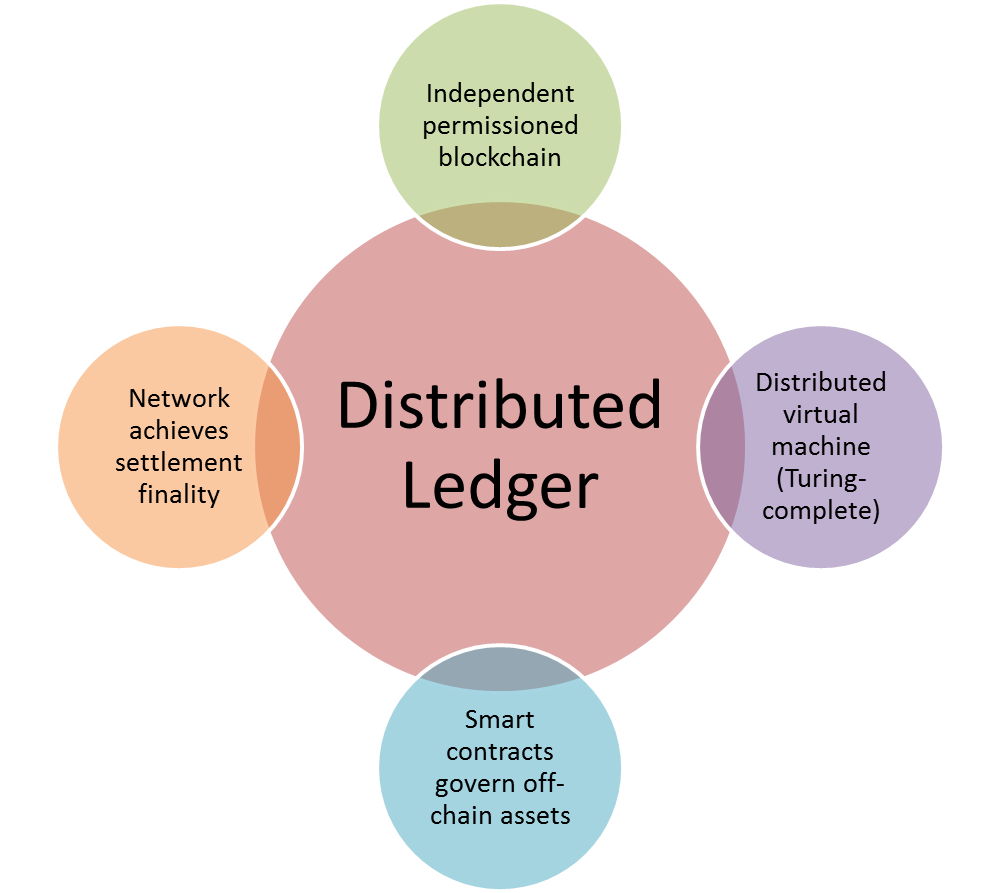
\includegraphics[scale=0.35]{./images/dlt}
        \end{column}
    \)
\end{frame}

%%%%%%%%%%%%%%%%%%%%%%%%%%%%%%%%%%%%%%%%%%%%%%%%%%%%%%
%%%%%%%%%%%%%%%%%%%%%%%%%%%%%%%%%%%%%%%%%%%%%%%%%%%%%%
\subsection{Definitions}
\begin{frame}{definitions}
    \begin{itemize}
        \item Distributed Ledger vs BlockChain
        \item Target user
        \item Electronic signature
        \item Asymmetrical cryptography
    \end{itemize}
\end{frame}


%%%%%%%%%%%%%%%%%%%%%%%%%%%%%%%%%%%%%%%%%%%%%%%%%%%%%%
%%%%%%%%%%%%%%%%%%%%%%%%%%%%%%%%%%%%%%%%%%%%%%%%%%%%%%
\section{\scshape Problems} % Problem statement
\subsection{Modern problems and questions}
\begin{frame}{problems}
\begin{itemize}
        \item Existing classification expired
        \item Lack of technical information
        \item Bad blockchain creators programms
\end{itemize}
\end{frame}


%%%%%%%%%%%%%%%%%%%%%%%%%%%%%%%%%%%%%%%%%%%%%%%%%%%%%%
%%%%%%%%%%%%%%%%%%%%%%%%%%%%%%%%%%%%%%%%%%%%%%%%%%%%%%
\section{\scshape Methodology}
\subsection{Theoretical and practical approaches}
\begin{frame}{methodology}
    \begin{itemize}
        \item Literature review
        \item Benchmark analysis
        \item Programming using Python 3.6.5
    \end{itemize}
\end{frame}


%%%%%%%%%%%%%%%%%%%%%%%%%%%%%%%%%%%%%%%%%%%%%%%%%%%%%%
%%%%%%%%%%%%%%%%%%%%%%%%%%%%%%%%%%%%%%%%%%%%%%%%%%%%%%
\section{\scshape Expected results}
\subsection{Concluding above}
\begin{frame}{expected results}
    \begin{itemize}
        \item Structured body of knowledge is helpful
        \item Research provides an in-depth view
        \item Python library is used by target users
    \end{itemize}
\end{frame}

%%%%%%%%%%%%%%%%%%%%%%%%%%%%%%%%%%%%%%%%%%%%%%%%%%%%%%
%%%%%%%%%%%%%%%%%%%%%%%%%%%%%%%%%%%%%%%%%%%%%%%%%%%%%%
\section{\scshape References}
\subsection{Sources and literature used}
\begin{frame}{sources and literature used}
\begin{thebibliography}{1}
\tiny
\bibitem {swanson}
Swanson, T., \emph{Great Chain of Numbers: A Guide to Smart Contracts,
Smart Property and Trustless Asset Management.}, 2014, pp.44-47.

\bibitem {scientific}
Xu, Xiwei \& Weber, Ingo \& Staples, Mark \& Zhu, Liming \& Bosch, Jan \& Bass,
Len \& Pautasso, Cesare \& Rimba, Paul. \emph{A Taxonomy of Blockchain-Based Systems for
Architecture Design.}, 2017, 10.1109/ICSA.2017.33, pp. 4-6.

\bibitem {nakamoto}
Nakamoto, S. \emph{Bitcoin: A Peer-to-Peer Electronic Cash System}, 2014.
[ebook] Available at: \url{https://bitcoin.org/bitcoin.pdf} [Accessed 9 Feb. 2019].

\bibitem {ripple}
Schwartz, D., Youngs,N., Britto, A., \emph{The Ripple Protocol Consensus Algorithm}, 2014.
[ebook] Available at: \url{https://ripple.com/files/ripple_consensus_whitepaper.pdf} [Accessed 9 Feb. 2019].

\bibitem {iota}
The IOTA Foundation, \emph{IOTA whitepaper}, 2016.
[ebook] Available at: \url{http://iotatoken.com/IOTA_Whitepaper.pdf} [Accessed 9 Feb. 2019].

\bibitem {plasma}
Poon, J., Buterin, V., \emph{Plasma: Scalable Autonomous Smart Contracts}, 2017.
[ebook] Available at: \url{https://plasma.io/plasma.pdf} [Accessed 9 Feb. 2019].

\bibitem {verge}
Sunerock, J. \emph{Blackpaper}, 2019.
[ebook] Available at: \url{https://vergecurrency.com/static/blackpaper/verge-blackpaper-v5.0.pdf}, 5th ed., [Accessed 9 Feb. 2019].

\bibitem {tkey}
TKEY DMCC, \emph{TKEYCOIN TECHNICAL DESIGN DOCUMENTATION}, 2018.
[ebook] Available at: \url{https://tkeycoin.com/docs/whitepaper/whitepaper.pdf}, [Accessed 9 Feb. 2019].
\end{thebibliography}
\end{frame}


%%%%%%%%%%%%%%%%%%%%%%%%%%%%%%%%%%%%%%%%%%%%%%%%%%%%%%
%%%%%%%%%%%%%%%%%%%%%%%%%%%%%%%%%%%%%%%%%%%%%%%%%%%%%%
\section{\scshape Questions}
% \subsection{Questions}
\begin{frame}{questions}
Any questions?
\end{frame}


\section{}
%%%%%%%%%%%%%%%%%%%%%%%%%%%%%%%%%%%%%%%%%%%%%%%%%%%%%%
%%%%%%%%%%%%%%%%%%%%%%%%%%%%%%%%%%%%%%%%%%%%%%%%%%%%%%
\begin{frame}{Thank you for attention}
    \underline{Contacts}\\

    \vspace{0.5cm}
    Kirill I. Kupriyanov\\
    \emph{mephisto@openmail.cc}\\

    \vspace{0.3cm}
    Sergey M. Avdoshin\\
    \emph{savdoshin@hse.ru}
\end{frame}

\end{document}


% EOF

